We will be using vectors for calculating the area of the triangle formed by above three points.
%
\begin{align}
    \Vec{B-A} =\myvec{
    2\\3
    } -\myvec{
    -1\\2}
\end{align}
    
\begin{align} \label{2/2/6/eq1}
\Vec{B-A}= \myvec{3\\1}
\end{align}
\begin{align}
\Vec{C-A} =\myvec{
4\\-3
} -\myvec{
-1\\2 }
\end{align}
\begin{align} \label{2/2/6/eq2}
\Vec{C-A}= \myvec{5\\-5}
\end{align}
\begin{align} \label{2/2/6/eq3}
    \because
    \text{Area of the Triangle}  = \frac{1}{2}\norm {(\Vec{B-A})\times ( \Vec{C-A}) }
\end{align}
\newline

As the vector cross product of two vectors can also be expressed as the product of a skew-symmetric matrix and a vector.

\begin{align} \label{2/2/6/eq4}
    \Vec{P}\times  \Vec{Q}  = 
    \myvec{
    0&-a_{3}&a_{2}\\
    a_{3}&0&-a_{1}\\
    -a_{2}&a_{1}&0\\
    }
    \times \myvec{
    b_{1}\\
    b_{2}\\
    b_{3}\\}
\end{align}
Substituting values from equation \eqref{2/2/6/eq1} and \eqref{2/2/6/eq2} in above equation \eqref{2/2/6/eq4}, we'll get:

\begin{align}
    \Vec{(B-A)}\times  \Vec{(C-A)}  = 
    \myvec{
    0&0&1\\
    0&0&-3\\
   -1&3&0\\}
    \times \myvec{
    5\\
    -5\\
    0\\}
\end{align}
\begin{align} \label{2/2/6/eq5}
    \Vec{(B-A)}\times  \Vec{(C-A)}  = \myvec{
    0\\
    0\\
    -20\\}
\end{align}
\begin{align} \label{2/2/6/eq5}
\frac{1}{2}    \therefore \norm {\Vec{(B-A)}\times  \Vec{(C-A)} }  = 10
\end{align}
Substituting value from equation \eqref{2/2/6/eq5} in equation \eqref{2/2/6/eq3}, we'll get area of triangle:

$
\implies  \frac{1}{2}(20) =10 units^2
$
\begin{figure}[!h]
\centering
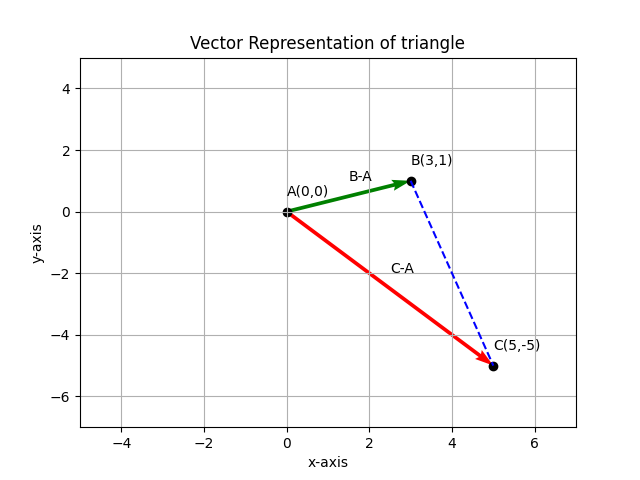
\includegraphics[width=\columnwidth]{solutions/2/2/6/image(graph).png}
\caption{Plot obtained from Python code}
\label{2/2/6/Fig:1}
\end{figure}

